\chapter{Volatility}
\label{chapter:volatility}
As mentioned, volatility is a measure of the uncertainty of future stock price movements. In other words, a higher volatility will lead to greater future fluctuations in the stock price, whereas a stock with lower volatility is more stable. This phenomenon is exemplified in \autoref{fig:VarVol}, where we can see the greater fluctuations of the high-volatility process (red) compared to the much smaller variations of the low-volatility process (orange), using the same driving Brownian motion.
\begin{figure}[!htb]
    \centering
      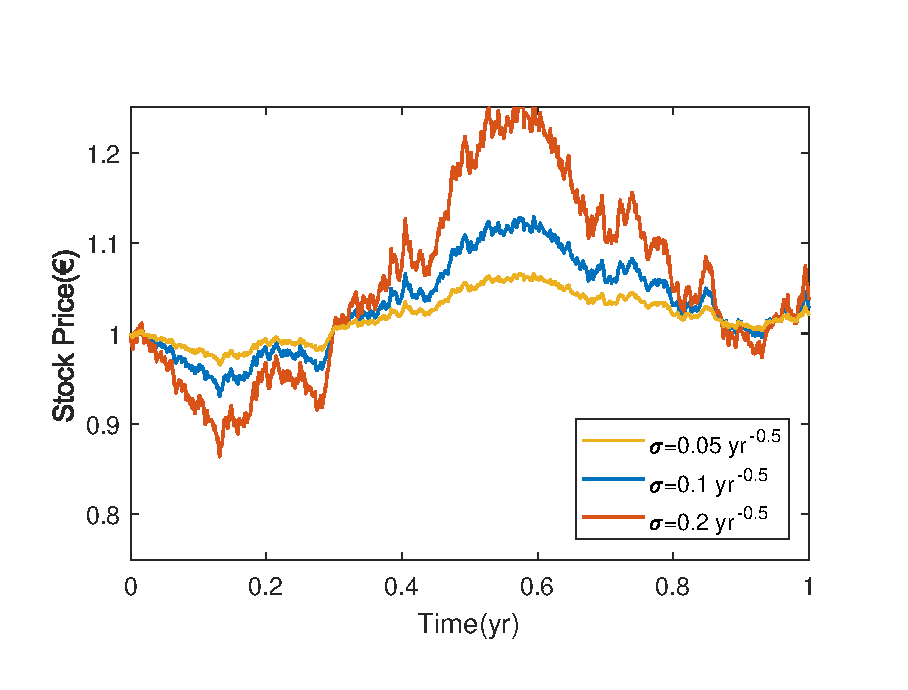
\includegraphics[width=.65\columnwidth]{VarVol.eps}
      \caption[Example of three identical GBM processes with different volatilities]{Example of three identical GBM processes with maturity $T=1\SI{}{\year}$, interest rate $r=0.01\SI{}{\per\year}$ and initial stock price $S_0=1\SI{}{\EUR}$. The volatilities are $\sigma=0.05\SI{}{\year\tothe{-1/2}}$, $\sigma=0.1\SI{}{\year\tothe{-1/2}}$ and $\sigma=0.2\SI{}{\year\tothe{-1/2}}$ for the orange, blue and red plot lines represented, respectively. To emphasize this effect, the underlying Brownian Motion $\{W(t),\ t>0\}$ used to generate all three paths was the same.}\label{fig:VarVol}
    \end{figure}

\section{Why Volatility is Important}
\label{section: Why Volatility is Important}
Volatility is of the utmost importance when trading options. We can show that the greater the volatility of a stock, the higher the price of its corresponding option. 
To understand why option price increases with volatility we can note that volatility is very desirable to investors when dealing with options. A high volatility means that there is an increased probability that the stock price will increase or decrease very significantly. In the case of a call option, if the stock price increases considerably, the investor earns a large amount of money. If the price decreases considerably, the investor may let the option expire, thus avoiding further losses. Thus we see that a higher volatility provides a greater change of potentially very high profits with a limited potential downfall. We thus conclude that a higher volatility increases the value of an option and this parameter has a great influence on the option price.
Furthermore, of all the parameters in the BS formula (eq.\eqref{BS2}), volatility is the only one we can't easily measure from market data.
These two factors make volatility one of the most important subjects in all of mathematical finance and thus the focus of much research.




\section{Estimating Volatility}
Usually, volatility can be estimated empirically from the standard deviation of the historical rate of log-returns~\citep{Hull}.
We begin by measuring the stock price at fixed time intervals (e.g. daily, monthly), such that $S_i$ corresponds to the stock price at the end of the $i$th interval. We define the log-return rate, $u_i$, as
\begin{equation}
u_i=\log\left(\frac{S_i}{S_{i-1}}\right).
\end{equation}
We can then calculate the standard deviation, $s$, of this rate as
\begin{equation}
s=\sqrt{\frac{1}{n-1}\sum_{i=1}^n(u_i-\overline{u})^2},
\end{equation}
\noindent assuming we have $n+1$ observations and denoting $\overline{u}$ as the average value of the log-return rates.
The volatility (measured yearly) can be \emph{estimated} with
\begin{equation}
\hat{\sigma}=\frac{s}{\sqrt{\tau}},
\end{equation}
\noindent where $\tau$ defines the time interval length measured in years. As an example, if we only have monthly data for the $S_i$ prices, the time interval would obviously be one month, which, measured in years is equal to $1/12$, which corresponds to $\tau$.
The volatility can also be measured in other time periods: we can define a monthly or a daily volatility, instead of a yearly volatility as we defined before, but these are less common and will therefore not be used.

We are now able to estimate the volatility of any given asset at the present moment. With this result, we could assume that the volatilities remain constant over time and use today's volatility to price options with maturities in the future. The clear problem with this approach is that, when observing market data, we can see that \emph{volatilities change over time, so that even if we had the exact value of this parameter in the present, it can, and will, change in the future. If we try to price options assuming a constant volatility, our options will become mispriced, causing potential losses: volatility is itself a random process}.
Our goal is therefore to model the instantaneous volatility of any given stock price (i.e. its volatility at a given point in time), and, with this model, predict its future behavior, using this knowledge to better price options.
We begin by introducing the concept of implied volatility, crucial to fully grasping the concepts used later. Afterwards, we will introduce four models to replicate volatility: one using local volatility (Dupire's formula), where we assume that the volatility depends on the stock price and time (i.e. $\sigma_t=f(t,S_t)$), and three others using stochastic volatility (Heston and Static/Dynamic SABR), where the volatility also depends on a Brownian motion process (i.e. $\sigma_t=f(t,S_t,W_t^\sigma)$).

We should note that other very common models exist. The GARCH model~\citep{bollerslev} (Generalized Autoregressive Conditional Heteroskedasticity) along with all its many variations (EGARCH, NGARCH, ...) is particularly popular among econometricians. However, this model is mostly used to forecast volatility, and performs poorly when used to price derivatives~\citep{chourdakis}. Because pricing is our objective, GARCH will not be covered in this work. We will also study the constant volatility model, as used by Black \textit{et al.}, as a benchmark for the quality of our models.



\section{Implied Volatility}
\label{section:impliedvolatility}
\emph{Implied volatility} can be described as the value of stock price volatility that, when input into the BS pricer in eq.\eqref{callputBS}, outputs a value equal to the market price of a given option.
In other words, it would be the stock price volatility that the seller/buyer of the option used when pricing it (assuming the BS model was used).

We can also relate implied volatility to the volatility of the stock price as
\begin{equation}
\sigma_{imp}=\sqrt{\frac{1}{T}\int_0^T(\sigma(t))^2dt},
\end{equation}
\noindent where $\sigma_{imp}$ denotes the implied volatility and $\sigma(t)$ is the volatility of the stock price. Thus, the implied volatility can be thought of as the (root mean square) average of the volatility.

Because eq.\eqref{callputBS} is not explicitly invertible w.r.t. $\sigma$, we need to use some numerical procedure (e.g. Newton's method) to find the value of implied volatility that matches the market and model prices, i.e. we must find, numerically, the solution to the equation
\begin{equation}\label{impvolform}
C(\sigma_{imp})=C_{\mathrm{mkt}},
\end{equation}
\noindent where $C(\sigma_{imp})$ corresponds to the result of eq.\eqref{callputBS} using $\sigma_{imp}$ as (implied) volatility and $C_{\mathrm{mkt}}$ to the price of the call option observed in the market (it could also be the call option price resulting from a model or simulation).


We deduced in \autoref{section: Why Volatility is Important} that the relation between implied volatility and market option price is a monotonous increasing function.
This means that we can obtain the implied volatility of an option from its price and vice versa (i.e. the relationship is bijective). This duality is so fundamental that investors often disclose options by providing their implied volatility instead of their price~\citep{Wilmott}, as is indeed the case for the data we will use later to calibrate the models.



One important property of implied volatility is that, in the real-world, it depends on the strike price and the maturity. This should not occur in the "Black-Scholes world". Because the volatility is a property of the stock, if investors really used the the BS model to price their options, two options with the same underlying stock should have the same implied volatility, regardless of their strike prices or maturities (i.e. the same stock can't have two different volatilities at the same time).
However, when observing real market data, this is in fact what is observed.

The implied volatilities' dependence on the strike price can take one of two forms, known as \emph{smile} and \emph{skew}.
An implied volatility smile presents higher volatilities for options with strikes farther from the current stock price (i.e. the shape of a smile). A skew, on the other hand, only presents higher volatilities in one of these directions (i.e. only for strikes either greater or smaller than the current stock price). Both phenomena are represented in \autoref{fig:smileskew}.
\begin{figure}[!htb]
  \begin{subfigmatrix}{2}
    \subfigure[Smile]{\includegraphics[width=0.49\linewidth]{Smile.eps}}
    \subfigure[Skew]{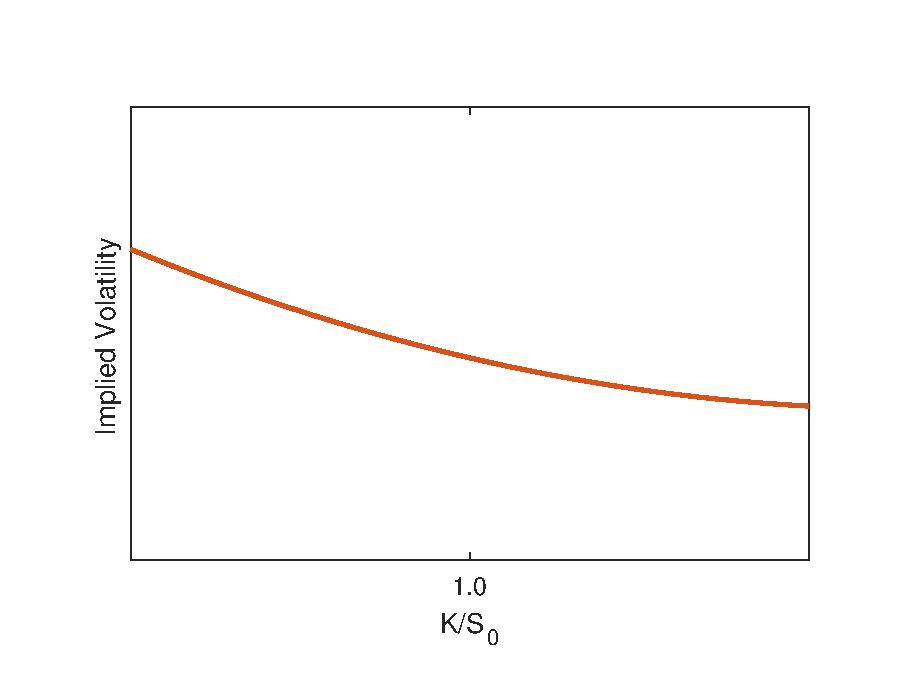
\includegraphics[width=0.49\linewidth]{Skew.eps}}
  \end{subfigmatrix}
  \caption[Representation of the implied volatility smile and skew functions.]{Representation of the implied volatility smile (left) and skew (right) functions.}
  \label{fig:smileskew}
\end{figure}


Because of their higher implied volatility, we can conclude that, if we observe a smile in the data, options with strikes different from the current stock price are \emph{overpriced}.
The reason behind this odd market behavior is related to the simple demand-supply rule~\citep{Wilmott3}. On the one hand, some investors are risk-averse and want to hedge their losses in case of a big market movement (as explained in \autoref{subsection:why options are important}). They don't mind paying a higher price for an option if this means they would be relatively safe from potentially devastating price changes. For this reason, the demand of call options with lower strikes increases, driving their prices and, consequently, their implied volatility up. On the other hand, other investors are risk-seekers and want to take advantage of possible sudden price movements, buying the stocks after the possible price increase for the lower strike prices. They don't mind paying higher prices for the chance of earning high profits and this drives the prices of high strike call options and, consequently, their implied volatility up. This fear-greed duality gives rise to the observed volatility smile. 
In the case of the volatility skew, only one of the two phenomena described occurs.


The presence of a smile in the data instead of a skew, and vice-versa, is determined by the type of product serving as underlying asset - Forex market options usually exhibit volatility smiles whereas index and commodities options usually show a volatility skew or a skewed smile~\citep{Wilmott3}.

The dependence of the implied volatility on the maturity date is more complex, but in general it decreases with the maturity.

In \autoref{fig:realimpliedvol} we plot an example of an implied volatility surface, along with its contour plot, which we obtained from real market data. This surface is again represented in \autoref{section:Dupire Model}. 
\begin{figure}[!htb]
  \begin{subfigmatrix}{2}
    \subfigure[Implied Volatility Surface]{\includegraphics[width=0.49\linewidth,trim={1.7cm 0.45cm 1.9cm 0.85cm},clip]{ImpVS.png}}
    \subfigure[Implied Volatility Contour Plot]{\includegraphics[width=0.49\linewidth,trim={0.2cm 0.5cm 1.25cm 1.55cm},clip]{ImpVSC.png}}
  \end{subfigmatrix}
  \caption[Representation of a real implied volatility surface and its respective contour plot.]{Representation of a real implied volatility surface and its respective contour plot.}
  \label{fig:realimpliedvol}
\end{figure}

As we can see from \autoref{fig:realimpliedvol} in this case we have a mixture of a smile and a skew behavior and the implied volatility does decrease with maturity, as expected.

It can also be shown that the implied volatility is the same for calls and puts~\citep{Hull}, though the causes of the volatility smile/skew for put options are the opposite of the ones described before for calls.

\iffalse
\hl{Though the implied volatility is usually defined for European options, we can just as easily adapt this term for Barrier options.} We again have to solve eq.\eqref{impvolform}, but now using the (Barrier) implied volatility, $\sigma_{imp,Barr}$, to generate the theoretical Barrier option price, $C(\sigma_{imp,Barr})$. This result will be used later when we study barrier options.
\fi

\section{Option Price Sensitivity and Vega}
\label{section:vega}
When studying volatilities, as is our case, one of the most important aspects to consider is the sensitivity of the option price to the volatility. In other words, we should try to understand how a small variation in the volatility of a given option affects its price. This sensitivity can be considered for other parameters, such as the interest rate or the maturity, but it is particularly important for the volatility because we don't actually know the exact value of this parameter. Therefore, if the option price is very sensitive to the volatility and we have a bad estimation for this parameter, we will have severe mispricing problems and possibly lose high amounts of money.

This sensitivity has been deeply studied in the literature and is usually called \emph{Vega}, or $\mathcal{V}$, and it is given by
\begin{equation}
\mathcal{V}=\pdv{V}{\sigma},
\end{equation}
\noindent where $V$ denotes the option price.
In particular for European calls, this value can be shown to be~\citep{Hull}
\begin{equation}
\mathcal{V}=S_0\sqrt{T}N'(d_1),
\end{equation}
\noindent where $d_1$ is given in eq.\eqref{d1d2} and $N'(\cdot)$ is the probability density function for a standard normal distribution.
If we plot this quantity against option strikes, we obtain the curve shown in \autoref{fig:Vega}.

\begin{figure}[H]
    \centering
      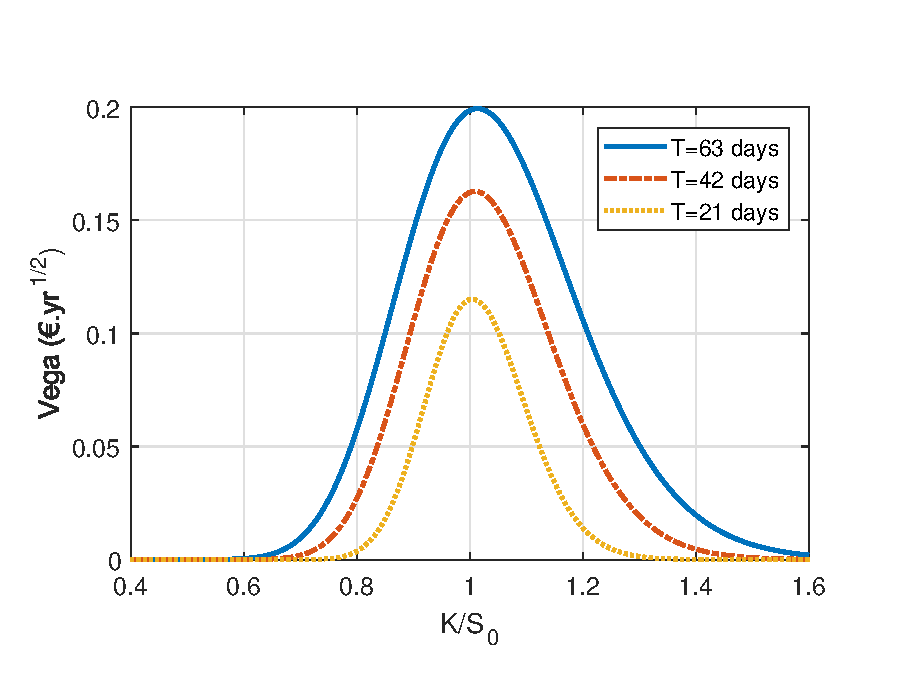
\includegraphics[width=.65\columnwidth]{Vega.eps}
      \caption[Relationship between the Vega and the respective options' strike prices, for different maturities.]{Relationship between the Vega and the respective options' strike prices, for different maturities. The parameters used were interest rate $r=0.01\SI{}{\per\year}$, initial stock price $S_0=1\SI{}{\EUR}$ and a constant volatility of $\sigma=0.3\SI{}{\year\tothe{-1/2}}$.}\label{fig:Vega}
    \end{figure}
    
As we can see, the Vega peaks when the strike equals the option price. This means that, at this point, a variation in the volatility will produce the largest variation on the corresponding strike price. Furthermore, we can see that this peak is more pronounced for later maturities.

Despite its usefulness, the Vega doesn't quite grasp the whole picture. As we said before, prices behave geometrically and not arithmetically - a change of $0.01\EUR$ in an option with price $0.5\EUR$ is quite different from the same change in an option with price $0.02\EUR$. A derivative (such as Vega) assumes arithmetic variations i.e. $\partial A/\partial B=0.1$ means that a change of 0.1 in $B$ produces a change of 1 in $A$. This doesn't contain any information on the \emph{relative change} of $A$ (i.e. if $A$ was an option price, we wouldn't know if it changed by $10\%$ or $0.1\%$).
To solve this shortcoming, we can simply define the \emph{relative change} as
\begin{equation}
\mathrm{Relative\ Change}=\pdv{V}{\sigma}\frac{\sigma}{V},
\end{equation}
\noindent which we plot in \autoref{fig:Vega2}, for call options, against their strike price.
As an example, if we have a relative change of $5$, this means that a variation of $1\%$ in the volatility will produce a variation of $5\%$ in the option price. 

\begin{figure}[H]
    \centering
      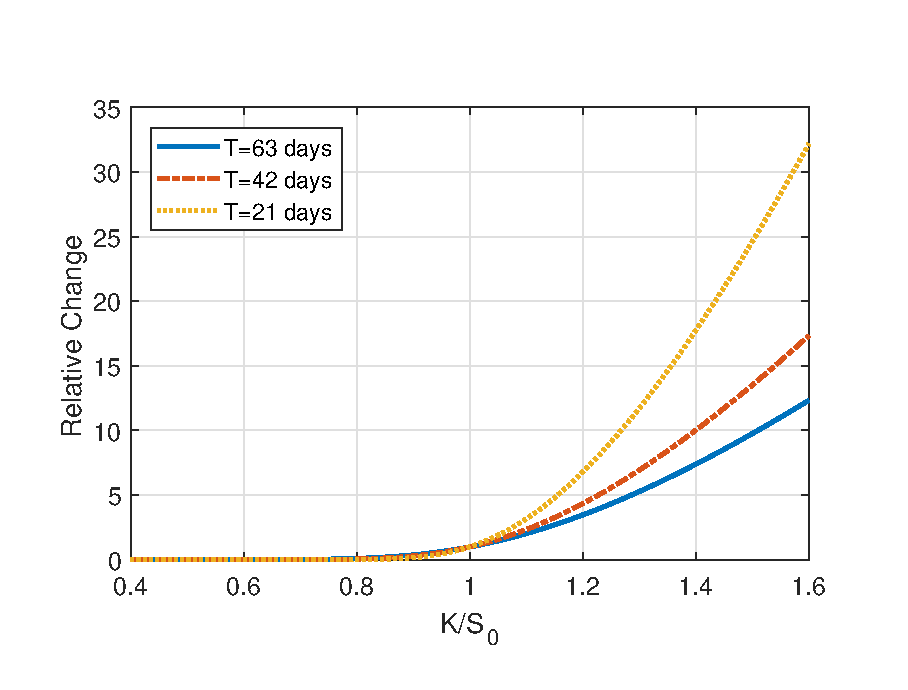
\includegraphics[width=.65\columnwidth]{Vega2.eps}
      \caption[Relationship between the (call) option price's relative change (w.r.t. volatility) and the respective strike prices, for different maturities.]{Relationship between the (call) option price's relative change (w.r.t. volatility) and the respective strike prices, for different maturities. The parameters used were interest rate $r=0.01\SI{}{\per\year}$, initial stock price $S_0=1\SI{}{\EUR}$ and a constant volatility of $\sigma=0.3\SI{}{\year\tothe{-1/2}}$.}\label{fig:Vega2}
    \end{figure}
    
As we can see in \autoref{fig:Vega2}, the relative change of the option price w.r.t. volatility is very large for call options with high strikes. We can therefore conclude that the prices of options with high strikes are very sensitive to the value of volatility. This implies that a very slight (relative) change in the volatility will produce a very large (relative) change in the option price. It also means that the volatility is very robust w.r.t. the option price ,i.e. a very large (relative) variation in the option price will barely affect the volatility. We will observe this effect in later sections.

The opposite effect is found for call options with lower strikes - we can see that the relative variation of the option price w.r.t. the volatility is extremely small in these cases, meaning that the option price is extremely robust to the volatility, i.e. a change in the volatility will affect the option price only very slightly. It also implies that the volatility is extremely sensitive to the option price, meaning that a very slight (relative) change in the price of a call option with low strikes will dramatically change its volatility. This observation will become very important in later sections.

Furthermore, we can also observe that the relative change of the option price w.r.t. the volatility is greater for options with smaller maturities, which will also be observed later.

For later comparison, we note that the value of relative change of the option price w.r.t. the volatility is approximately $1$ when $K=S_0$ for all maturities.

\section{Local Volatility}
\label{section:localvolatility}
In their original work, Black \textit{et al.} assumed that volatility is constant throughout the whole option duration~\citep{Scholes}. From market data, it can be clearly seen that this is not the case~\citep{DJIA}. There may be times when new information reaches the market  (e.g. the results of an election) and trading increases, driving volatility up. It is equally true that shortly before this information is known, trading may stall due to expectancy, and volatilities go down.

The constant volatility BS model is therefore clearly insufficient of completely grasping real-world trading. We should use a model where volatility is dynamic, measuring the uncertainty on the stock price movement at any point in time.
However, as we saw in \autoref{section:impliedvolatility}, the market's view of volatility also depends on the stock price itself.
The volatility should therefore be a function of both time and stock price: $\sigma(S(t),t)$. We call this model \emph{local volatility} and the geometric Brownian motion from eq.\eqref{GBM} is transformed into the new diffusion process
\begin{equation}\label{GBM2}
dS(t)=rS(t)dt+\sigma(S(t),t)S(t)dW(t),
\end{equation}
\noindent where $\sigma(S(t),t)$ is a function of $S(t)$ and $t$, with certain properties, which we omit as they are only used to ensure the strong solution of this SDE (i.e. $\sigma(S(t),t)$ is "well behaved").


This local volatility model implies that we have a nonlinear \emph{deterministic} volatility surface, $\sigma(S(t),t)$, which can be thought of as the market's expectation of future volatility at time $t$ if the stock price is $S(t)$ at that time.



Because we can't directly measure the local volatility of a stock from market data, we need some models to estimate it. One of the most used of these is known as Dupire's formula, which we explain in the following subsection.


\subsection{Dupire's model}
\label{subsection:Dupire}
One of the most famous results in the modelling of the local volatility function was obtained by Dupire~\citep{Dupire}. In his article, this author derives a theoretical formula for $\sigma(S(t),t)$, given by
\begin{equation}\label{dupire}
\sigma(S(t),t)=\sqrt{\frac{\displaystyle\pdv{C}{T}+rS\pdv{C}{K}}{\displaystyle\frac{1}{2}S^2\pdv{^2C}{K^2}}},
\end{equation}
\noindent where $C=C(K,T)$ is the price of an European call option with strike price $K$ and maturity $T$. All the derivatives are evaluated at $K=S(t)$ and $T=t$.



\begin{proof}

We begin by assuming that the stock price $S(t)$ follows a dynamic transition probability density function $p(S(t),t,S'(t'),t')$. In other words, by integrating this density function we would obtain the probability of the stock price reaching a price $S'$ at a time $t'$ having started at price $S$ at time $t$.

The present value of a call option, $C(K,T)$, can be deduced as its expected future payoff, discounted backwards in time, which results in
\begin{equation}
\begin{split}\label{deriv0}
C(K,T)=e^{-r(T-t)}\mathbb{E}\left[\max\left(S'-K,0\right)\right]&=e^{-r(T-t)}\int_0^\infty\max\left(S'-K,0\right)p(S,t,S',T)dS'\\
&=e^{-r(T-t)}\int_K^\infty(S'-K)p(S,t,S',T)dS',
\end{split}
\end{equation}
\noindent where $S'$ denotes the stock price at maturity.

Taking the first derivative of this result with respect to the strike price $K$, we obtain
\begin{equation}\label{dcdk}
\pdv{C}{K}=-e^{-r(T-t)}\int_K^\infty p(S,t,S',T)dS'.
\end{equation}
The second derivative results in
\begin{equation}\label{d2cdk2}
\pdv{^2C}{K^2}=e^{-r(T-t)}p(S,t,K,T),
\end{equation}
\noindent assuming $p(S,t,\infty,T)=0$.

We now make a brief digression to derive the Fokker-Planck equation (following the procedure shown in Wilmott~\citep{Wilmott3}), which we require for the next steps. This equation is widely used in stochastic calculus, and is applicable to stochastic processes in general.
To make its proof simpler, we make a simplification assuming that the stochastic process is a stock price following a trinomial model: at each time step $\delta t$, the stock price can only increase or decrease by an amount $\delta S$, with probabilities $\phi^+$ and $\phi^-$, respectively, or remain the same, with probability $(1-\phi^+-\phi^-)$. The resulting equation still works, however, for any general stochastic process.


Assuming the trinomial model, the expected value of the change is given by
\begin{equation}
\phi^+\delta S+(1-\phi^+-\phi^-).0+\phi^-(-\delta S)=(\phi^+-\phi^-)\delta S,
\end{equation}
\noindent and its variance is approximately given by
\begin{equation}
(\delta S)^2(\phi^++\phi^--(\phi^+-\phi^-)^2)\approx (\phi^++\phi^-)(\delta S)^2
\end{equation}
\noindent where we take only the first order terms. The expected value of the change of a Geometric Brownian Motion can be thought of as its drift term (i.e. $rS\delta t$), and the variance is its stochastic term squared (i.e. $(\sigma SdW)^2=\sigma^2S^2\delta t$), so that we have
\begin{equation}
\begin{split}
rS\delta t&=(\phi^+-\phi^-)\delta S;\\
\sigma^2S^2\delta t&=(\phi^++\phi^-)(\delta S)^2,
\end{split}
\end{equation}
\noindent from which we can derive the probabilities $\phi^+$ and $\phi^-$ as
\begin{equation}
\begin{split}
\phi^+(S,t)&=\frac{1}{2}\frac{\delta t}{\delta S^2}(rS\delta S+\sigma^2S^2);\\
\phi^-(S,t)&=\frac{1}{2}\frac{\delta t}{\delta S^2}(-rS\delta S+\sigma^2S^2).
\end{split}
\end{equation}

We can now move backwards and derive the probability of reaching the price $S'$ at time $t'$ having started at the previous time $t'-\delta t$ with some (unknown) price $S$, which could be either $S'+\delta S$, $S'-\delta S$ or $S'$ (assuming a trinomial movement). Applying the same logic as before, the probability of reaching $S'$ at time $t'$, having started at $S$ at time $t$, is the same as the probability of being at $S'-\delta S$ at time $t'-\delta t$ and moving up, plus the probability of being at $S'+\delta S$ at time $t'-\delta t$ and moving down plus the probability of being at $S'$ at time $t'-\delta t$ and remaining at the same value. We can thus derive the transition probability density, $ p(S,t,S',t')$ as
\begin{equation}
\begin{split}
p(S,t,S',t')=&\phi^-(S'+\delta S,t'-\delta t)p(S,t,S'+\delta S,t'-\delta t)\\
&+(1-\phi^+(S',t'-\delta t)-\phi^-(S',t'-\delta t))p(S,t,S',t'-\delta t)\\
&+\phi^+(S'-\delta S,t'-\delta t)p(S,t,S'-\delta S,t'-\delta t)
\end{split}
\end{equation}
\noindent If we expand each term on its Taylor series around point $(S',t')$, we get
\begin{equation}
\begin{split}
p(S,t,S',t')=&\ \phi^-(S'+\delta S,t'-\delta t)\left(p(S,t,S',t')+\delta S\pdv{p}{S'}+\frac{1}{2}(\delta S)^2\pdv{^2p}{S^2}-\delta t\pdv{p}{t'}\right)\\
&+(1-\phi^+(S',t'-\delta t)-\phi^-(S',t'-\delta t))\left(p(S,t,S',t')-\delta t\pdv{p}{t'}\right)\\
&+\phi^+(S'-\delta S,t'-\delta t)\left(p(S,t,S',t')-\delta S\pdv{p}{S'}+\frac{1}{2}(\delta S)^2\pdv{^2p}{S^2}-\delta t\pdv{p}{t'}\right),
\end{split}
\end{equation}
\noindent from which, collecting all the terms, we can derive the famous Fokker-Planck equation~\citep{Wilmott3} (with rather sloppy notation) as
\begin{equation}\label{FokkerPlanck}
\pdv{p}{T}=\frac{1}{2}\pdv{^2(\sigma^2S'^2p)}{S'^2}-\pdv{(rS'p)}{S'}.
\end{equation}
\noindent where we have used $t'=T$.


From eq.\eqref{deriv0} we can easily obtain the first derivative w.r.t. time
\begin{equation}
\pdv{C}{T}=-rC+e^{-r(T-t)}\int_K^\infty(S'-K)\pdv{p}{T}dS',
\end{equation}
\noindent where, for simplicity, we drop the terms of the transition probability density, $p$.

Using the Fokker-Planck formula in eq.\eqref{FokkerPlanck}, we can transform this relation into
\begin{equation}
\pdv{C}{T}=-rC+e^{-r(T-t)}\int_K^\infty(S'-K)\left(\frac{1}{2}\pdv{^2(\sigma^2S'^2p)}{S'^2}-r\pdv{(S'p)}{S'}\right)dS'.
\end{equation}

We now split the terms in the integral to evaluate them independently. We integrate the second term by parts as
\begin{equation}
\begin{split}
\int_K^\infty(S'-K)\left(-r\pdv{(S'p)}{S'}\right)dS'&=-r(S'-K)(S'p)\big|_{S'=K}^\infty+r\int_K^\infty S'p dS'\\
&=r\int_K^\infty (S'-K)p dS'+rK\int_K^\infty p dS'\\
&=e^{r(T-t)}rC-rK\pdv{C}{K}
\end{split}
\end{equation}
\noindent where in the first step we assumed that $p$ and its first derivative w.r.t. $S$ go sufficiently fast to zero when $S$ goes to infinity and where in last step we used eqs.\eqref{deriv0} and\eqref{dcdk}.

Turning now to the first term of the integral, we integrate twice by parts as
\begin{equation}
\begin{split}
\int_K^\infty(S'-K)\left(\frac{1}{2}\pdv{^2(\sigma^2S'^2p)}{S'^2}\right)dS'&=\frac{1}{2}(S'-K)\pdv{(\sigma^2S'^2p)}{S'}\bigg|_{S'=K}^\infty-\frac{1}{2}\int_K^\infty\left(\pdv{(\sigma^2S'^2p)}{S'}\right)dS'\\
&=-\frac{1}{2}\sigma^2S'^2p\big|_{S'=K}^\infty=\frac{1}{2}\sigma^2(K,T)K^2p(S,t,K,T)\\
&=\frac{1}{2}e^{r(T-t)}\sigma^2(K,T)K^2\pdv{^2C}{K^2},
\end{split}
\end{equation}
\noindent where in the last step we used eq.\eqref{d2cdk2} and again assumed that $p$ goes to zero sufficiently fast.

Collecting all the terms, we obtain
\begin{equation}
\pdv{C}{T}=\frac{1}{2}\sigma^2(K,T)K^2\pdv{^2C}{K^2}-rK\pdv{C}{K}.
\end{equation}
\noindent from which, by rearranging all the terms and applying the variable change $\sigma(K,T)\implies \sigma(S,t)$, we get
\begin{equation}
\sigma(S(t),t)=\sqrt{\frac{\displaystyle\pdv{C}{T}+rS\pdv{C}{K}}{\displaystyle\frac{1}{2}S^2\pdv{^2C}{K^2}}}.
\end{equation}
\noindent assuming all the derivatives are evaluated at $K=S(t)$ and $T=t$.

\end{proof}

As can be seen, we need to differentiate the option prices with respect to their strikes and maturities. To achieve this, we need first to gather, from the market, a large number of prices for options with different maturities and strikes. We then implement some interpolation on these values to obtain an option price surface (with $K$ and $T$ as variables). Finally, we calculate the gradients of this interpolated surface and input them into eq.\eqref{dupire} to obtain the local volatility surface.
We can then sample from this surface to obtain the local volatility for any stock price $S(t)$ at any time $t$.


A major problem can be pointed out in eq.\eqref{dupire}. For options far in or far out of the money (i.e. with strikes much greater or much smaller that $S_0$), it can be shown that the option price depends almost linearly on the strike. This means that the second derivative of the price w.r.t. the strike is extremely small in these regions. Because this value is in the denominator of eq.\eqref{dupire}, the local volatility will explode in such cases, which is unrealistic.


One possible solution to this problem is to relate our local volatility with the implied volatility surface instead of the option price's~\citep{Wilmott}.
The relation obtained is
\begin{equation}\label{dupire2}
\boxed{\sigma(S(t),t)=\sqrt{\frac{\displaystyle\sigma_{imp}^2+2t\sigma_{imp}\pdv{\sigma_{imp}}{T}+2r(S(t))t\sigma_{imp}\pdv{\sigma_{imp}}{K}}{\displaystyle\left(1+(S(t))d_1\sqrt{t}\pdv{\sigma_{imp}}{K}\right)^2+(S(t))^2t\sigma_{imp}\left(\pdv{^2\sigma_{imp}}{K^2}-d_1\left(\pdv{\sigma_{imp}}{K}\right)^2\sqrt{t}\right)}},}
\end{equation}
\noindent where $d_1$ is given by
\begin{equation}
d_1=\frac{\log(S_0/S(t))+\left(r+\frac{1}{2}\sigma_{imp}^2\right)t}{\sigma_{imp}\sqrt{t}},
\end{equation}
\noindent with $S_0$ being the stock price at $t=0$. We define $\sigma_{imp}=\sigma_{imp}(K,T)$ as the implied volatilities of options with maturity $T$, and strike $K$. Furthermore, $\sigma_{imp}$ and all its derivatives are evaluated at $K=S(t)$ and $T=t$. This formula can be obtained from eq.\eqref{dupire} by applying the transformation from call prices to implied volatilities.


We now need to generate the implied volatility surface in order to obtain the gradients needed in eq.\eqref{dupire2} to generate the local volatility. Again, this surface can be obtained by interpolating between market data for several implied volatilities. The problem with this approach is that we only have access to market data for a very limited set of implied volatilities. This problem is therefore very much ill-posed (i.e. a small change in the input generates a very different output) and the resulting local volatility surface might look unrealistic~\citep{Wilmott}. Furthermore, this procedure is heavily dependent on the interpolation/extrapolation method chosen, which is problematic.

As an advantage, we note that because we are directly using the market data, the implied volatility surface is nonparametric and therefore no fitting procedure is required. To ease the problem of ill-posedness, we could heuristically choose some functions to model this surface, fitting their parameters to better replicate the market data, and finally replacing these functions in eq.\eqref{dupire2}, as done by Dewynne~\citep{dewynne}. However, this solution depends heavily on the functions chosen and will not be considered.



Three other problems can be identified in Dupire's local volatility model.
First, it can be shown that the local volatility surface changes with time~\citep{Wilmott}. This means that the whole interpolation procedure must be done regularly in order for the model to work properly.
Secondly, some authors have pointed out that the volatility smile obtained from Dupire's local-volatility model doesn't follow real market dynamics~\citep{Hagan}: it can be shown that when the price of the stock either increases or decreases, the volatility smile predicted by Dupire's model shifts in the opposite direction. The minimum of the volatility smile would therefore be offset and no longer correspond to the local stock price (i.e. the spot price). The volatility smile dynamics obtained from the local-volatility model would thus be actually worse than if we assumed a constant volatility.
Finally, the gradients used in eq.\eqref{dupire2} have to be generated numerically. This numerical differentiation is very unstable, especially when done on our rough interpolated surface, which might lead to errors in the local volatility obtained.

As an example, in \autoref{fig:LocVol} we show a local volatility surface, obtained by applying Dupire's formula to real data, along with its corresponding contour plot. This surface will again be represented in \autoref{section:Dupire Model} and studied with greater detail there.
\begin{figure}[!htb]
  \begin{subfigmatrix}{2}
    \subfigure[$\sigma_{loc}$ surface]{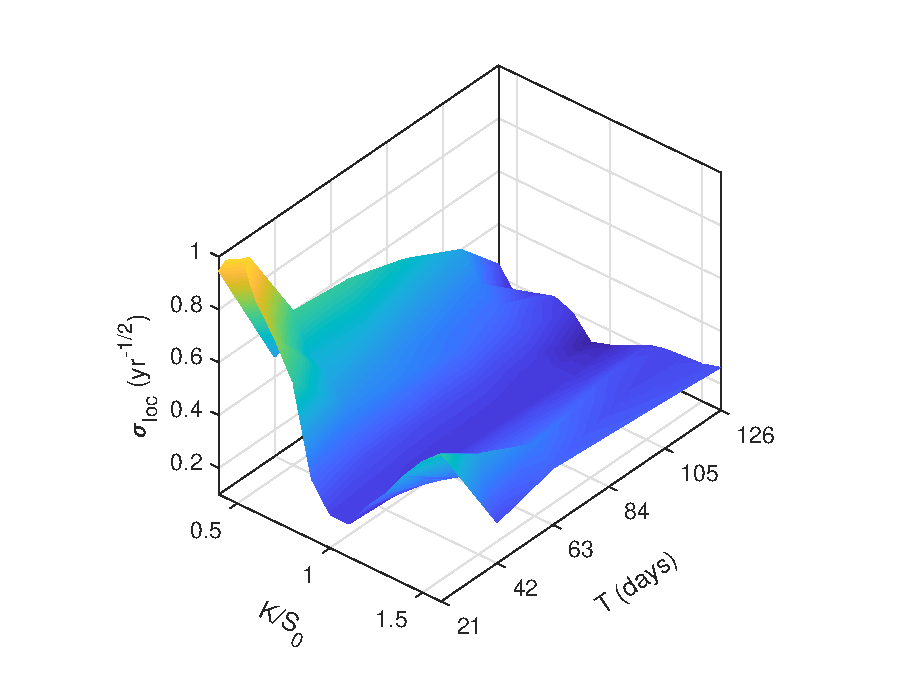
\includegraphics[width=0.49\linewidth,trim={1.7cm 0.45cm 2.cm 0.85cm},clip]{LocalV.eps}}
    \subfigure[$\sigma_{loc}$ contour plot]{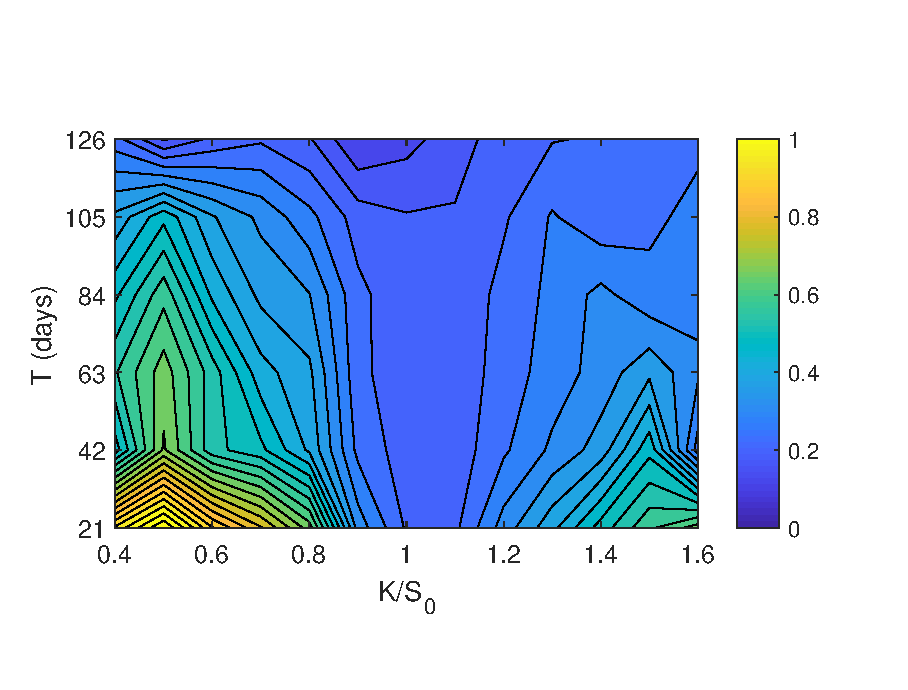
\includegraphics[width=0.49\linewidth,trim={0.2cm 0.5cm 1.25cm 1.55cm},clip]{LocalVC.eps}}
  \end{subfigmatrix}
    \caption[Example of a real local volatility surface and corresponding contour plot.]{Example of a real local volatility surface and corresponding contour plot.}\label{fig:LocVol}
\end{figure}  

Despite its problems, Dupire's formula is still very much used by practitioners and performs surprisingly well, as we will see in \autoref{chapter:results}.



\section{Stochastic Volatility}
\label{section:stochastic volatility}
As stated before, the volatility is not constant, is not observable and is very unpredictable, despite our attempts to model it. This seems to indicate that volatility is itself also a stochastic process~\citep{rebonato}. Some research has been done into this hypothesis, and many models have been developed to replicate real-world volatilities with this assumption.

We assume that the stock price follows the diffusion process
\begin{equation}\label{stochvol}
dS(t)=rS(t)dt+\sigma(S(t),t)S(t)dW_1(t),
\end{equation}
\noindent and we further hypothesize that the volatility follows
\begin{equation}
d\sigma(S(t),t)=p(S(t),\sigma(S(t),t),t)dt+q(S(t),\sigma(S(t),t),t)dW_2(t),
\end{equation}
\noindent where $p(S(t),\sigma(S(t),t),t)$ and $q(S(t),\sigma(S(t),t),t)$ are functions of the stock price $S(t)$, time $t$ and of the volatility $\sigma(S(t),t)$ itself. We also assume that $W_1$ and $W_2$ are two Brownian motion processes with a correlation $\rho(t)$, i.e.
\begin{equation}
dW_1(t)dW_2(t)=\rho(t) dt, \ \ \ \forall t>0,
\end{equation}
\noindent which is usually assumed constant, $\rho(t)=\rho$. This correlation coefficient can be explained by the relationship between prices and volatilities~\citep{chourdakis}. Historically, we can see that high volatility periods usually occur when the market is under stress due to low returns (i.e. stock prices decrease).
On the other hand, whenever the market stabilizes and returns increase, the volatility goes down.
These factors seem to indicate the existence of a negative correlation between stock prices and volatilities. Thus, to fully grasp market behavior, this correlation must be taken into account.



Choosing the appropriate functions $p(S(t),\sigma(S(t),t),t)$ and $q(S(t),\sigma(S(t),t),t)$ is very important since the whole evolution of the stock price depends on them. All stochastic volatility models present a different version of these functions, and each may be more adequate for some types of assets. Furthermore, these functions have some parameters that we have to calibrate in order to best fit our model to market data, as we will see later.


Many stochastic volatility models exist, such as Hull-White~\citep{hullwhite} and Stein-Stein~\citep{stein}. However, the \emph{Heston} model is by far the most popular of these~\citep{chourdakis}.
Another model, known as \emph{SABR}, is also widely used by practitioners, especially in the interest rate derivative markets (i.e. derivatives whose underlying asset is an interest rate). For these reasons, both these models will be studied in this work.


\subsection{Heston Model}
The \emph{Heston model} was developed in 1993 by Steven Heston~\citep{Heston} and it states that stock prices satisfy the relations
\begin{subequations}
\begin{empheq}[box=\widefbox]{align}
&dS(t)=rS(t)dt+\sqrt{\nu(t)}S(t)dW_1(t),\label{hestons}\\
&d\nu(t)=\kappa(\overline{\nu}-\nu(t))dt+\eta\sqrt{\nu(t)}dW_2(t),\label{hestonv}
\end{empheq}
\end{subequations}
\noindent with $\nu(t)$ corresponding to the stock price variance (i.e. the square of the volatility, $\nu(t)=(\sigma(t))^2$) and where $W_1(t)$ and $W_2(t)$ have a constant correlation $\rho$. We furthermore define $\nu_0$ as the initial variance (i.e. variance at time $t=0$). The original model used a drift parameter $\mu$ instead of the risk-free measure drift $r$ presented here, but a measure transformation, using Gisarnov's theorem, can be easily implemented~\citep{rouah}.

The parameters $\kappa$, $\overline{\nu}$ and $\eta$ are, respectively, the \emph{mean-reversion rate} (i.e. how fast the variance converges to its mean value), the \emph{long-term variance} (i.e. the mean value of variance) and the \emph{volatility of the variance} (i.e. how erratic is the variance process).



One of the reasons why the Heston model is so popular is the fact that there exists a closed-form solution for the prices of European options priced under this model. This closed form solution is given by
\begin{equation}\label{CH}
\begin{split}
C_{H}(K,T;\theta)&=e^{-rT}\mathbb{E}\left[\left(S(T)-K\right)\mathbbm{1}_{\left\{S(T)>K\right\}}\ \vert\ \theta\right]\\
&=e^{-rT}\left(\mathbb{E}\left[S(T)\mathbbm{1}_{\left\{S(T)>K\right\}}\ \vert\ \theta\right]-K\mathbb{E}\left[\mathbbm{1}_{\left\{S(T)>K\right\}}\ \vert\ \theta\right]\right)\\
&=S_0P_1(K,T;\theta)-e^{-rT}KP_0(K,T;\theta),
\end{split}
\end{equation}
\noindent where $C_{H}(K,T;\theta)$ corresponds to the theoretical European call option price, with strike $K$ and maturity $T$, under the Heston model, assuming a parameter set $\theta=\left\{\kappa,\overline{\nu},\eta,\nu_0,\rho\right\}$. The variables $P_1(K,T;\theta)$ and $P_2(K,T;\theta)$ are given by
\begin{equation}\label{P1}
P_1(K,T;\theta)=\frac{1}{2}+\frac{1}{\pi}\int_0^\infty\operatorname{Re}\left(\frac{e^{-iu\log K}}{iuS_0e^{rT}}\phi(u-i,T;\theta)\right)du,
\end{equation}
\begin{equation}\label{P2}
P_0(K,T;\theta)=\frac{1}{2}+\frac{1}{\pi}\int_0^\infty\operatorname{Re}\left(\frac{e^{-iu\log K}}{iu}\phi(u,T;\theta)\right)du,
\end{equation}
\noindent where $i$ is the imaginary unit and $\phi(u,t;\theta)$ is the characteristic function of the logarithm of the stock price process (the characteristic function of a random variable is the Fourier transform of the probability density function of that variable).


It is crucial to define the appropriate characteristic function $\phi(u,t;\theta)$ in order to evaluate the integrals in eqs.\eqref{P1} and\eqref{P2} and, with them, find the option price with eq.\eqref{CH}. In his original article, Heston proposed a solution to this very characteristic function~\citep{Heston}. However, some posterior authors demonstrated that, for large maturities, some discontinuities appeared for the proposed solution~\citep{Kahl}. One possible alternative, proposed by Schoutens~\citep{Schoutens}, avoids this shortcoming and is given by
\begin{equation}\label{charfuncschoutens}
\phi(u,t;\theta)=\exp\left\{iu\left(\log S_0+rt\right)+\frac{\kappa\overline{\nu}}{\eta^2}\left[\left(\xi-\alpha\right)t-2\log\left(\frac{1-ge^{-\alpha t}}{1-g}\right)\right]+\frac{\nu_0}{\eta^2}\left(\xi-\alpha\right)\frac{1-e^{-\alpha t}}{1-ge^{-\alpha t}}\right\},
\end{equation}
\noindent where we define
\begin{equation}\label{xi}
\xi=\kappa-\eta\rho iu,
\end{equation}
\begin{equation}\label{alpha}
\alpha=\sqrt{\xi^2+\eta^2(u^2+iu)},
\end{equation}
\begin{equation}
g=\frac{\xi-\alpha}{\xi+\alpha}.
\end{equation}


\begin{proof}
We will follow the derivation presented in Gatheral~\citep{gatheral} with slight changes of variables, for consistency.

We begin by defining Itô's Lemma for a function $V$ (such as the price of an option) dependent on the behavior of two diffusion processes $X$ and $Y$ (such as the stock price and variance processes, but also applicable to two different stock price processes), which is given by
\begin{equation}
dV=\pdv{V}{t}dt+\pdv{V}{X}dX+\pdv{V}{Y}dY+\frac{1}{2}\sigma_X^2\pdv[2]{V}{X}dt+\rho\sigma_X\sigma_Y\pdv{V}{X}{Y}dt+\frac{1}{2}\sigma_Y^2\pdv[2]{V}{Y}dt,
\end{equation}
\noindent where we have assumed that the two diffusion processes are defined as
\begin{equation}
\begin{split}
&dX=\mu_X(X,Y,t)dt+\sigma_X(X,Y,t)dW_X;\\
&dY=\mu_Y(X,Y,t)dt+\sigma_Y(X,Y,t)dW_Y,
\end{split}
\end{equation}
\noindent where $W_X$ and $W_Y$ have a correlation of $\rho$.

If we apply this lemma (as well as the usual non-arbitrage arguments) to the price of a call option's value, assuming the diffusion processes to be the stock price and variance defined in eqs.\eqref{hestons} and \eqref{hestonv}, we arrive at
\begin{equation}\label{hestonproof1}
\pdv{C}{t}+\frac{1}{2}\nu S^2\pdv[2]{C}{S}+\rho\eta\nu S\pdv{C}{\nu}{S}+\frac{1}{2}\eta^2\nu\pdv[2]{C}{\nu}+rS\pdv{C}{S}-rC+\kappa(\overline{\nu}-\nu)\pdv{C}{\nu}=0.
\end{equation}

We now define the forward price as $F(t)=S(t)e^{r(T-t)}$, and introduce the variables $\tau=T-t$ and $x(t)=\log\left(F(t)/K\right)$. We furthermore denote $C^*$ as the future value to expiration of the option price (i.e. $C^*=Ce^{rT}$). The relation in eq.\eqref{hestonproof1} reduces to
\begin{equation}\label{hestonproof2}
-\pdv{C^*}{\tau}+\frac{1}{2}\nu\pdv[2]{C^*}{x}+\rho\eta\nu\pdv{C^*}{x}{\nu}+\frac{1}{2}\eta^2\nu\pdv[2]{C^*}{\nu}-\frac{1}{2}\nu\pdv{C^*}{x}+\kappa(\overline{\nu}-\nu)\pdv{C^*}{\nu}=0,
\end{equation}
\noindent which has a solution of the form ~\citep{duffie}
\begin{equation}\label{hestonproof3}
C^*(x,\nu,\tau)=Ce^{rT}=\left(S_0P_1-e^{-rT}KP_0\right)e^{rT}=K\left[e^xP_1(x,\nu,\tau)-P_0(x,\nu,\tau)\right].
\end{equation}


Substituting the solution of eq.\eqref{hestonproof3} in eq.\eqref{hestonproof2} implies that $P_0$ and $P_1$ must satisfy
\begin{equation}\label{hestonproof4}
-\pdv{P_j}{\tau}+\frac{1}{2}\nu\pdv[2]{P_j}{x}-\left(\frac{1}{2}-j\right)\nu\pdv{P_j}{x}+\frac{1}{2}\eta^2\nu\pdv[2]{P_j}{\nu}+\rho\eta\nu\pdv{P_j}{x}{\nu}+\left(\kappa(\overline{\nu}-\nu)+j\nu\rho\eta\right)\pdv{P_j}{\nu}=0,
\end{equation}
\noindent for $j=0,1$ and subject to the terminal condition $P_j(x,\nu,\tau=0)=\mathbbm{1}_{\left\{x>0\right\}}$.


To solve this problem we use a Fourier transform technique. Defining $\tilde{P_j}$ as the Fourier transform of $P_j$,
\begin{equation}
\tilde{P_j}(u,\nu,\tau)=\int_{-\infty}^{\infty}e^{-iux}P_j(x,\nu,\tau)dx,
\end{equation}
\noindent and substituting this result in eq.\eqref{hestonproof4} produces
\begin{equation}\label{hestonproof5}
\nu\left\{\omega_j\tilde{P_j}-\beta_j\pdv{\tilde{P_j}}{\nu}+\frac{\eta^2}{2}\pdv[2]{\tilde{P_j}}{\nu}\right\}+\kappa\overline{\nu}\pdv{\tilde{P_j}}{\nu}-\pdv{\tilde{P_j}}{\tau}=0,
\end{equation}
\noindent with
\begin{equation}
\omega_j=-\frac{u^2}{2}-\frac{iu}{2}+iju,
\end{equation}
\begin{equation}
\beta_j=\kappa-\rho\eta iu-\rho\eta j.
\end{equation}


Heston proposed that $\tilde{P_j}$ is a function of the form
\begin{equation}
\tilde{P_j}(u,\nu,\tau)=\frac{1}{iu}\exp\left\{\zeta_j(u,\tau)\overline{\nu}+\psi_j(u,\tau)\nu\right\}.
\end{equation}

We can therefore derive
\begin{equation}
\pdv{\tilde{P_j}}{\tau}=\left\{\overline{\nu}\pdv{\zeta_j}{\tau}+\nu\pdv{\psi_j}{\tau}\right\}\tilde{P_j},
\end{equation}
\begin{equation}
\pdv{\tilde{P_j}}{\nu}=\psi_j\tilde{P_j},
\end{equation}
\begin{equation}
\pdv[2]{\tilde{P_j}}{\nu}=\psi_j^2\tilde{P_j}.
\end{equation}

Thus, eq.\eqref{hestonproof5} is only satisfied if
\begin{equation}
\pdv{\zeta_j}{\tau}=\kappa\psi_j,
\end{equation}
\begin{equation}
\pdv{\psi_j}{\tau}=\omega_j-\beta_j\psi_j+\frac{\eta^2}{2}\psi_j^2.
\end{equation}

Integrating these solutions with terminal conditions $\zeta_j(u,0)=\psi_j(u,0)=0$, yields
\begin{equation}
\zeta_j(u,\tau)=\frac{\kappa}{\eta^2}\left[\left(\beta_j-\gamma_j\right)\tau-2\log\left(\frac{1-g_je^{-\gamma_j \tau}}{1-g_j}\right)\right],
\end{equation}
\begin{equation}
\psi_j(u,\tau)=\frac{1}{\eta^2}\left(\beta_j-\gamma_j\right)\frac{1-e^{-\gamma_j \tau}}{1-g_je^{-\gamma_j \tau}},
\end{equation}
\noindent where we define
\begin{equation}
\gamma_j=\sqrt{\beta_j-2\omega_j\eta^2},
\end{equation}
\begin{equation}
g_j=\frac{\beta_j-\gamma_j}{\beta_j+\gamma_j}.
\end{equation}

We finally arrive at the solution for $P_j$ given by
\begin{equation}
P_j(x,\nu,\tau)=\frac{1}{2}+\frac{1}{\pi}\int_0^\infty\operatorname{Re}\left(\frac{\exp\left\{\zeta_j(u,\tau)\overline{\nu}+\psi_j(u,\tau)\nu+iux\right\}}{iu}\right)du.
\end{equation}

A change of variables is possible, as shown by Crisostomo~\citep{Crisostomo}, such that the two different characteristic functions for $P_1$ and $P_0$ can be transformed into a single one by defining
\begin{equation}
P_1=\frac{1}{2}+\frac{1}{\pi}\int_0^\infty\operatorname{Re}\left(\frac{e^{-iu\log K}}{iuS_0e^{rT}}\phi(u-i,T;\theta)\right)du,
\end{equation}
\begin{equation}
P_0=\frac{1}{2}+\frac{1}{\pi}\int_0^\infty\operatorname{Re}\left(\frac{e^{-iu\log K}}{iu}\phi(u,T;\theta)\right)du,
\end{equation}
\noindent with the characteristic function $\phi(u,T;\theta)$ given by
\begin{equation}
\phi(u,t;\theta)=\exp\left\{iu\left(\log S_0+rt\right)+\frac{\kappa\overline{\nu}}{\eta^2}\left[\left(\xi-\alpha\right)t-2\log\left(\frac{1-ge^{-\alpha t}}{1-g}\right)\right]+\frac{\nu_0}{\eta^2}\left(\xi-\alpha\right)\frac{1-e^{-\alpha t}}{1-ge^{-\alpha t}}\right\}.
\end{equation}

\end{proof}



The main problem with the characteristic function presented in eq.\eqref{charfuncschoutens} is the fact that it is highly nonlinear. Because we will apply some optimization procedure to minimize the difference between the model and the market option prices (i.e. calibration), the optimizer is very likely become stuck in some local minimum and not find the globally optimal solution.
This shortcoming led some authors to propose several modified versions of this function, such as Rollin \textit{et al.}~\citep{Rollin}. Most recently, Cui \textit{et al.}~\citep{Cui} presented a characteristic function that not only doesn't have the previously mentioned discontinuities but also solves the nonlinearity problem, given by
\begin{equation}
\phi(u,t;\theta)=\exp\left\{iu\left(\log S_0+rt\right)-\frac{t\kappa\overline{\nu}\rho iu}{\eta}-\nu_0A+\frac{2\kappa\overline{\nu}}{\eta^2}D\right\},
\end{equation}
\noindent with $A$ and $D$ given by
\begin{equation}
A=\frac{A_1}{A_2},
\end{equation}
\begin{equation}
D=\log \alpha+\frac{(\kappa-\alpha) t}{2}-\log\left(\frac{\alpha+\xi}{2}+\frac{\alpha-\xi}{2}e^{-\alpha t}\right),
\end{equation}
\noindent where $\xi$ and $\alpha$ are given by eqs.\eqref{xi} and\eqref{alpha}, respectivelly, and where we introduce the variables $A_1$, $A_2$, given by
\begin{equation}
A_1=(u^2+iu)\sinh\frac{\alpha t}{2},
\end{equation}
\begin{equation}
A_2=\alpha\cosh\frac{\alpha t}{2}+\xi\sinh\frac{\alpha t}{2}.
\end{equation}

With this result we are now able to find the prices of options under the Heston model for a given set of parameters $\theta$. We just need to calibrate the parameters to some market data to be able to model the volatility process.

\subsubsection{Negative Variance and Feller's Condition}
One last consideration is required for the Heston model.
By analyzing eqs.\eqref{hestons} and \eqref{hestonv} we can see that the square root of the variance is used. This shouldn't pose a problem, since the variance of any process is always positive. However, because in our case this variable is itself stochastic, we must guarantee that it doesn't become negative, or else the square root would output imaginary numbers. To ensure this, we can apply Feller's condition~\citep{feller} and force the parameters to obey
\begin{equation}
2\kappa\overline{\nu}>\eta^2.
\end{equation}
\noindent However, this condition restricts the reachable space of our model. One possible alternative is to set the variance to zero every time it becomes negative:
\begin{equation}
\nu=\max\left[\nu^*,0\right],
\end{equation}
\noindent where $\nu^*$ corresponds to the unrestricted variance and $\nu$ is the new (always positive) variance, ensuring that the square root outputs a real number. Because this alternative allows any value for the parameters, it will be adopted in the implementation of the Heston model.


\subsection{Static SABR Model}
One other very famous model for stochastic volatility was developed by Hagan \textit{et al.}~\citep{Hagan} and is known as \emph{SABR} - we will henceforth refer to it by \emph{Static SABR}, to distinguish it from the \emph{Dynamic SABR} model that we will see next. SABR stands for "\emph{stochastic-}$\alpha\beta\rho$" and in this model it is assumed that the option prices and volatilities follow~\citep{Geeske}
\begin{subequations}
\begin{empheq}[box=\widefbox]{align}
&dS(t)=rS(t)dt+e^{-r(T-t)(1-\beta)}\sigma(t)(S(t))^\beta dW_1(t),\label{dF}\\
&d\sigma(t)=\nu\sigma(t) dW_2(t),\label{dsigma}
\end{empheq}
\end{subequations}
\noindent where we define $\alpha=\sigma(0)$ as the starting volatility and $S_0=S(0)$ as the starting stock price. Furthermore, as before, the two Brownian motion processes $W_1(t)$ and $W_2(t)$ have a \emph{constant} correlation of $\rho$.

The parameters $\beta$ and $\nu$ correspond, respectively to the \emph{skewness} (i.e. how the volatility smile moves when the stock price changes) and the \emph{volatility of volatility} (i.e. how erratic is the volatility process).



In the original article, the authors claim that $\beta$ can be fitted from historical market data, but usually investors choose this value heuristically, depending on the type of assets traded. Typical values used are $\beta=1$ (stochastic lognormal model), used for foreign exchange options, $\beta=0$ (stochastic normal model), typical for interest rate options and $\beta=0.5$ (stochastic CIR model), also common for interest rate options~\citep{Hagan}.
Because are trying to compare several models, we will make no assumptions on the data used. Therefore, we will leave this parameter free when fitting the model to the market data, assuming no heuristics.

One of the main problems with the static SABR model is the fact that, unlike the Heston model, the stochastic volatility process is not mean-reverting. This shortcoming enables the volatility to evolve unrestrictedly which is problematic - it may become negative, which is clearly absurd, or it may become extremely large, which is troublesome. Labordère~\citep{Labordere} proposed a mean-reverting correction to static SABR, but we will study the original model by Hagan \textit{et al.}, as it is more commonly used. We should still note that while negative volatilities make no sense in the real world, by examining eq.\eqref{dF} we can see that this should pose no problem upon simulations, since this effect would be equivalent to inverting the Brownian motion process (i.e. $dW(t)\implies-dW(t)$), which is obviously allowed.

One of the main reasons why static SABR is so popular is due to its quasi-closed-form solutions that enable us to quickly find the implied volatilities of options priced under this model. With the corrections done by Oblój on Hagan's original formula~\citep{Obloj}, it can be shown that these implied volatilities are given by
\begin{equation}\label{sabr}
\begin{split}
\sigma_{SABR}(K,f,T)\approx&\frac{1}{\displaystyle\left[1+\frac{(1-\beta)^2}{24}\log^2\left(\frac{f}{K}\right)+\frac{(1-\beta)^4}{1920}\log^4\left(\frac{f}{K}\right)\right]}.\left(\frac{\nu\log\left(f/K\right)}{x(z)}\right)\\
&.\left\{1+T\left[\frac{(1-\beta)^2}{24}\frac{\alpha^2}{(Kf)^{1-\beta}}+\frac{1}{4}\frac{\rho\beta\nu\alpha}{(Kf)^{(1-\beta)/2}}+\frac{2-3\rho^2}{24}\nu^2\right]\right\},
\end{split}
\end{equation}
\noindent with $z$ and $x(z)$ defined as
\begin{equation}
z=\frac{\nu\left(f^{1-\beta}-K^{1-\beta}\right)}{\alpha(1-\beta)},
\end{equation}
\begin{equation}
x(z)=\log\left\{\frac{\sqrt{1-2\rho z+z^2}+z-\rho}{1-\rho}\right\},
\end{equation}
\noindent where we have used $f=S_0e^{rT}$. The proof of this solution is quite lengthy and will not be replicated here, though it can be found in the original article~\citep{Hagan}.

For the particular case where $f=K$, evaluating eq.\eqref{sabr} produces a $0/0$ indeterminate form. This poses no problem because the closed form solution actually simplifies to~\citep{Hagan}
\begin{equation}
\sigma_{SABR}(K,f=K,T)\approx\frac{\alpha}{K^{1-\beta}}.\left\{1+T\left[\frac{(1-\beta)^2}{24}\frac{\alpha^2}{K^{2(1-\beta)}}+\frac{1}{4}\frac{\rho\beta\nu\alpha}{K^{1-\beta}}+\frac{2-3\rho^2}{24}\nu^2\right]\right\}.
\end{equation}

As for the Heston model, we again need to calibrate the parameters of this model to be able to model the volatility process.


\subsection{Dynamic SABR Model}
\label{subsection:Dynamic SABR Model}
One of the main setbacks of the static SABR model is the fact that it should only be calibrated on a set of options with the same maturity. The model behaves badly when we try to fit options with different maturities~\citep{Hagan}. 

To solve this problem, Hagan \textit{et al.} suggested a similar model known as \emph{Dynamic SABR}~\citep{Hagan}. It follows the same diffusion processes presented in eqs.\eqref{dF} and\eqref{dsigma} but with time-dependent parameters $\rho(t)$ and $\nu(t)$,
\begin{subequations}
\begin{empheq}[box=\widefbox]{align}
&dS(t)=rS(t)dt+e^{-r(T-t)(1-\beta)}\sigma(t)(S(t))^\beta dW_1(t),\label{dF2}\\
&d\sigma(t)=\nu(t)\sigma(t) dW_2(t),\label{dsigma2}
\end{empheq}
\end{subequations}
\noindent with the correlation between $W_1(t)$ and $W_2(t)$ now given by
\begin{equation}
dW_1(t)dW_2(t)=\rho(t) dt, \ \ \ \forall t>0.
\end{equation}
\noindent where $\rho(t)$ is now a function of time.



Hagan \textit{et al.} derived again a quasi-closed-form solution for the implied volatilities of options priced under this model. Osajima later simplified this expression using asymptotic expansion~\citep{Osajima}. The resulting formula is given by
\begin{equation}\label{dynsabr}
\sigma_{DynSABR}(K,f,T)=\frac{1}{\omega}\left(1+A_1(T)\log\left(\frac{K}{f}\right)+A_2(T)\log^2\left(\frac{K}{f}\right)+B(T)T\right),
\end{equation}
\noindent where $f=S_0e^{rT}$, $\ \omega=f^{1-\beta}/\alpha\ $ and where $A_1(T)$, $A_2(T)$ and $B(T)$ are given by
\begin{equation}
A_1(T)=\frac{\beta-1}{2}+\frac{\eta_1(T)\omega}{2},
\end{equation}
\begin{equation}
A_2(T)=\frac{(1-\beta)^2}{12}+\frac{1-\beta-\eta_1(T)\omega}{4}+\frac{4\nu_1^2(T)+3(\eta_2^2(T)-3\eta_1^2(T))}{24}\omega^2,
\end{equation}
\begin{equation}
B(T)=\frac{1}{\omega^2}\left(\frac{(1-\beta)^2}{24}+\frac{\omega\beta\eta_1(T)}{4}+\frac{2\nu_2^2(T)-3\eta_2^2(T)}{24}\omega^2\right),
\end{equation}
\noindent with $\nu_1^2(T)$, $\nu_2^2(T)$, $\eta_1(T)$ and $\eta_2^2(T)$ defined as
\begin{equation}\label{nu1}
\nu_1^2(T)=\frac{3}{T^3}\int_0^T(T-t)^2\nu^2(t)dt,
\end{equation}
\begin{equation}
\nu_2^2(T)=\frac{6}{T^3}\int_0^T(T-t)t\nu^2(t)dt,
\end{equation}
\begin{equation}
\eta_1(T)=\frac{2}{T^2}\int_0^T(T-t)\nu(t)\rho(t)dt,
\end{equation}
\begin{equation}\label{eta2}
\eta_2^2(T)=\frac{12}{T^4}\int_0^T\int_0^t\left(\int_0^s\nu(u)\rho(u)du\right)^2dsdt,
\end{equation}
\noindent where $\rho(t)$ and $\nu(t)$ are the functions chosen to model the time dependent parameters.


We now need to empirically choose some appropriate functions for $\rho(t)$ and $\nu(t)$.
We can choose these functions such that the integrals in eqs.\eqref{nu1}-\eqref{eta2} are analytically  solvable, greatly simplifying the calibration of this model. Hagan \textit{et al.} showed that the calibrated volatility of volatility, $\nu$, decreases with the maturity (in the Static SABR model)~\citep{Hagan}, which seems to suggest that the function $\nu(t)$ should decrease with time. As for the correlation parameter, $\rho$, these authors claimed that its time-dependent behavior is heavily dependent on the type of underlying asset traded. Using a stock index as the underlying asset (which is also the underlying asset for which we have data, shown in \autoref{chapter:mktdata}), Fernandez \textit{et al.} show that this parameter decreases (in absolute value) with maturity, indicating that $\rho(t)$ also decreases (in absolute value) with time~\citep{Fernandez}.
These authors thus suggest that we define $\rho(t)$ and $\nu(t)$ as
\begin{equation}\label{rhot}
\rho(t)=\rho_0e^{-at},
\end{equation}
\begin{equation}\label{nut}
\nu(t)=\nu_0e^{-bt},
\end{equation}
\noindent with $\rho_0\in[-1,1]$, $\nu_0>0$, $a>0$ and $b>0$.
In this particular case, $\nu_1^2(T)$, $\nu_2^2(T)$, $\eta_1(T)$ and $\eta_2^2(T)$ can be exactly derived as
\begin{equation}
\nu_1^2(T)=\frac{6\nu_0^2}{(2bT)^3}\left[\left(\frac{(2bT)^2}{2}-2bT+1\right)-e^{-2bT}\right],
\end{equation}
\begin{equation}
\nu_2^2(T)=\frac{12\nu_0^2}{(2bT)^3}\left[e^{-2bT}(1+bT)+bT-1\right],
\end{equation}
\begin{equation}
\eta_1(T)=\frac{2\nu_0\rho_0}{T^2(a+b)^2}\left[(a+b)T+e^{-(a+b)T}-1\right],
\end{equation}
\begin{equation}
\eta_2^2(T)=\frac{3\nu_0^2\rho_0^2}{T^4(a+b)^4}\left[e^{-2(a+b)T}-8e^{-(a+b)T}+(7+2T(a+b)(-3+(a+b)T))\right].
\end{equation}

There are other possible functions for $\rho(t)$ and $\nu(t)$. An example of such functions can be found in Fernandez \textit{et al.}~\citep{Fernandez}. The main concern with these functions is that they usually don't have analytically solvable solutions for the integrals in eqs.eqs.\eqref{nu1}-\eqref{eta2}, and these integrals need to be computed numerically, which greatly increases computation time. For this reason, they will not be considered in the present work.
